1\chapter{Introduction}

Zika virus is a member of the Flaviridae family
and the flavivirus genus, it is related to other mosquito borne viruses such as Dengue Virus, Yellow-Fever (YFV) virus  and West Nile virus \citep{doi}.The Virus originates from the Zika forest of Uganda and the first case was first isolated in 1947 from a rhesus monkey in the forest. Then later in 1954 a human was diagonised with the virus in Nigeria,\citep{2015zika}. Since then the virus has spread to different parts o the world. 
\begin{figure}[h!]
\centering
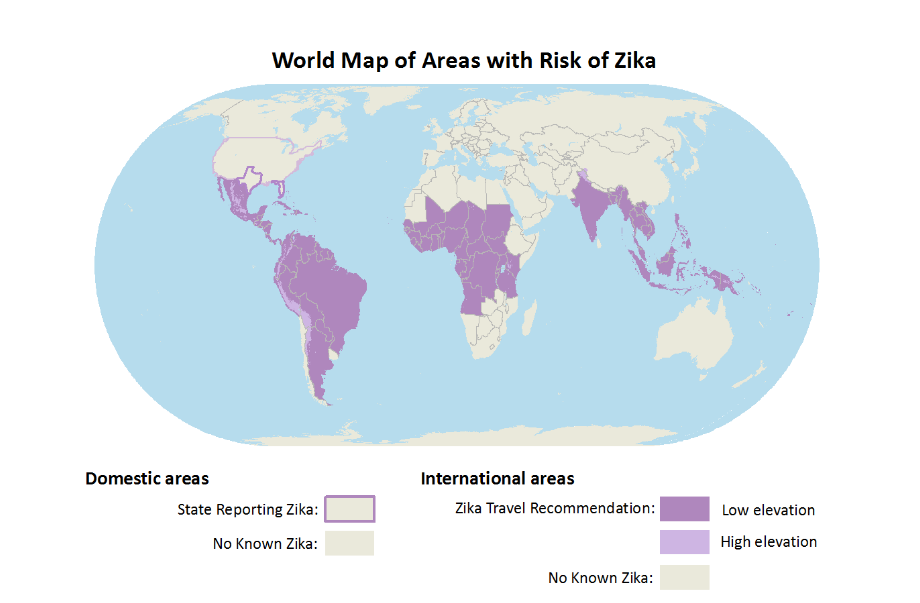
\includegraphics[scale=0.5]{images/map_zika.png} 
\caption{Counties with Zika Virus: Source CDC}\label{fig 1}
\end{figure}


Zika Virus is mainly spread by Aedes mosquitoes, when the Mosquito bites an infected person it carries the pathogen and when It bites an infected person it also it leaves the pathogen in them. Other ways of by which the virus spreads include, Blood transfusion, Unprotected Sex With an infected person and From mother to child, infected mothers can pass on the virus to their unborn children \citep{musso2014}.

\cite{musso2015}, shows that some of the symptoms are papular rash,fever,arthritis or arthralgia. In addition , headache, joint pain and red eyes are common symptoms of Zika virus. \cite{simoes2016zika} state adds that pregnant mothers who are infected with Zika during usually have child bearing defects. The Zika virus affect their foetus and development of the baby. Babies can face a range of neurologic sequelae suc as intellectual disability, hearing loss, vision loss, and seizures. These problems can range from mild to severe, are often life-long \citep{rasmussen2016zika}.

There is no known vaccination to prevent or treat for Zika virus. Prevention measures can be taken to prevent the spread of the virus. Preventing mosquito bites, this can be done by sleeping under a mosquito net, using mosquito replant, spraying mosquitos inside and outside among others. Another measure of prevention of Zika virus is practising safe sex and avoiding travelling to areas with high prevalence of Zika virus. Drugs for the systems of Zika are administered to patients as a way of treating Zika infected people because of the luck of a vaccination for the virus.


The spread of Zika virus has resulted in Zika epidemics in some part of the world as can be seen in figure \ref{fig 1} above. This cause a worry as the effects of an epidemic are more diver stating and if not controlled can affect the whole country region and World at large. 
 
 Mathematical models for disease transmission have been used to link biological processes of disease transmission and emergent of dynamics of infections at the population level. Researchers try to understand the environmental, biological  and behavioural infectiousness of a disease .
 
  Environmental infectiousness depends on geographical factors of an infected person. Some pathogens cannot survive inside or outside in given conditions. Thus some diseases or infections spread faster in certain weather conditions\citep{grass}. Understanding the timing and causes of seasonality offers important insights into how parasite–host systems interact how and when parasite control measures should be applied, and how disease risks will respond to anthropogenic climate change and altered patterns of seasonality \citep{altizer}. These factors must be captured in the models.
  
  Biological infectiousness depends on the pathogen's life cycle and the individual or host immune system. Some individuals have strong immune system against certain infections. This on the slows down the propagation the infection. On the other hand pathogens that live outside also affect the transmission dynamics of the infection.  The interaction of the genetic determinant of disease propagation in the pathogen and host is important in building model for the transmission dynamics of infectious diseases.
  
Behavioural infectiousness depends on the interaction behaviour of an individual. The contact pattern of the person affect how the individual is likely to propagate   the disease. Depending on the nature of disease transmission, if a persons has a lot of contact they are more likely to spread the disease to more people compared to one who has few contacts \citep{johnson2001sexual}. Contact in this context implies any interaction likely to result in the transmission of an infection.

The susceptibility of and individual largely depend on biological, environmental and behavioural factors of an individual. For example one's contact pattern, immunity and the environmental conditions will highly affect the probability of contracting an infection.

Epidemiologist together with mathematicians have for years been involved in infectious disease modelling to understand the dynamics of the spread of the disease and to come with measures of how the spread can be controls. Recently there has been a growing interest in modelling the spread of Zika virus \citep{ku2016}.

Over a  century, Mathematical representation and analysis of infectious diseases has been the centre of  infectious disease epidemiology \citep{b2005}. Differential equation have been used in the modelling of the dynamics of infectious diseases. They are base on the assumption of uniform mixing, that is everyone in the population has an equal probability of contracting an infectious disease \citep{kaplan2002emergency}.
Compartmental Mathematical models have been used to describe the transmission dynamic of Zika Virus \citep{gao2016}.

Graph theory has over the years grown and has found its application many fields. The concept of random graphs was first introduced by \cite{erdodblac1959ldquo}. A random graph can be defined as , given a $N$ number of vertices edges between them are drown such that between any pair $i,j$ there is an edge with uncorrelated probability $p$ \citep{newman2002random}. For example in \ref{fig:randomgraphs}, there are 3 random graphs with 10 vertices, with a probability of nodes $i,j$ being connect being 0, 0.5 and 0.8 in figure \ref{fig:a} \ref{fig:b} and \ref{fig:c} respectively.

\begin{figure}[h]
    \centering
    \begin{subfigure}[b]{0.3\textwidth}
        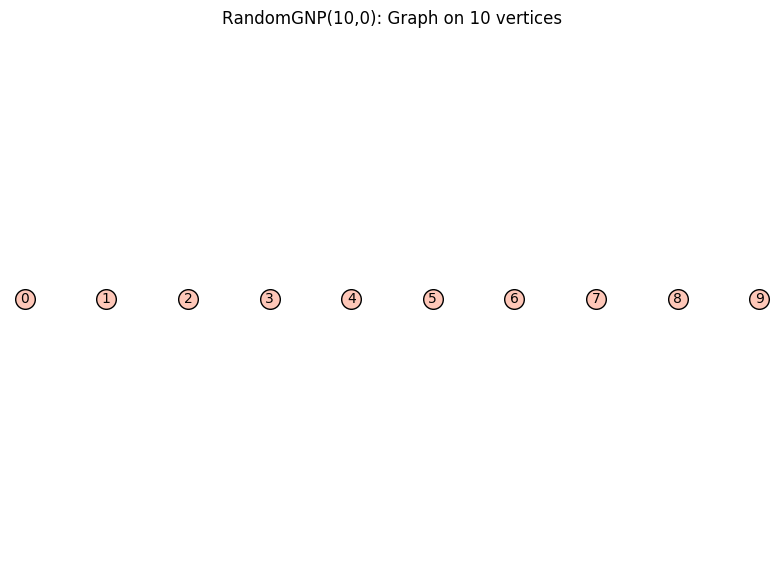
\includegraphics[scale=0.3]{images/rgraph2.png} 
        \caption{ $p =0$}
        \label{fig:a}
    \end{subfigure}
    ~ %add desired spacing between images, e. g. ~, \quad, \qquad, \hfill etc. 
      %(or a blank line to force the subfigure onto a new line)
    \begin{subfigure}[b]{0.3\textwidth}
        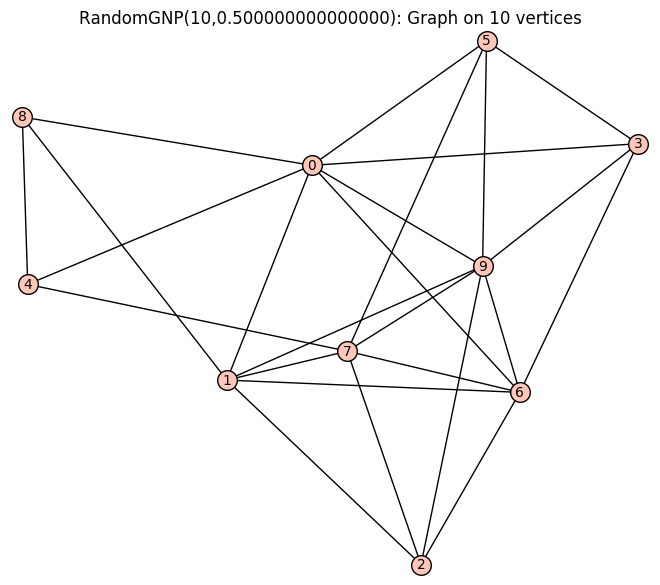
\includegraphics[width=\textwidth]{images/rgraph1.png}
        \caption{$p=0.5$}
        \label{fig:b}
    \end{subfigure}
    ~ %add desired spacing between images, e. g. ~, \quad, \qquad, \hfill etc. 
    %(or a blank line to force the subfigure onto a new line)
    \begin{subfigure}[b]{0.3\textwidth}
        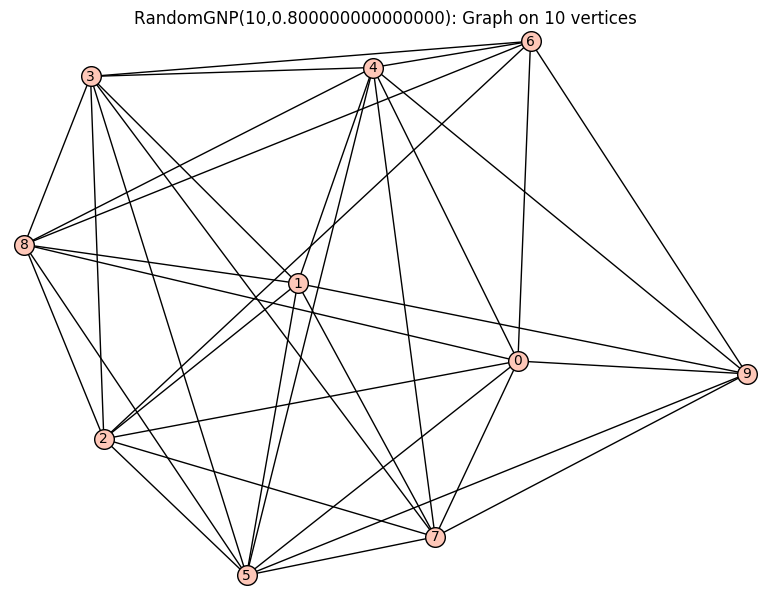
\includegraphics[width=\textwidth]{images/rgraph3}
        \caption{$p= 0.8$}
        \label{fig:c}
    \end{subfigure}
    \caption{Random Graphs}\label{fig:randomgraphs}
\end{figure}


The spread of disease in a community largely depends on the interaction of the individuals in a community. This can be expressed in a network, where each individual of the community is a vertex and when ever there is contact likely to result in the transmission of the disease an edge is drawn between any such nodes. Traditional epidemiological models , which the class of Susceptible, Exposed, Infectious, Recovered (SEIR) models are built on the assumption of random and uncorrelated mix in the population thus they form a random graph. $p$. 


  Small world networks, introduced by Strogatz and Watts, on the other
hand assume that one is more likely to spread the disease to someone in their family, someone
who lives near the, or someone you they. It combines this sort of clustering in the graph with a probability to model the spread of disease as a dynamical system \citep{newman2001random}.


In this research we will compare the traditional epidemiological model based on Random network assumption and the Small world networks to model the population Dynamics in the spread of Zika Virus. This infection of of Zika virus will be modelled using the SEIR compartmental model based on the two assumptions of transmission. Then real life data will be fit on both models to validate each model and to test which on is better.

